% =============================================================================
% Paper 1 — Present-epoch scale matching and C_obs hygiene on cubic T^3
% Genre: technical note (no-gos + one derived EFT identity)
% Class: Physical Review D (revtex4-2)
% =============================================================================
\documentclass[aps,prd,reprint,superscriptaddress,nofootinbib,floatfix,showkeys]{revtex4-2}

\usepackage[T1]{fontenc}
\usepackage[utf8]{inputenc}
\usepackage{amsmath,amssymb,amsthm}
\usepackage{booktabs}
\usepackage{graphicx}
\usepackage{hyperref}
\hypersetup{
  hidelinks,
  pdftitle={Present-epoch scale matching, the weak-field invariant Cobs, and constraints on a cubic T3 geometric construction},
  pdfauthor={Brendon Boyd},
  pdfkeywords={modified Newtonian dynamics, cosmic topology, effective field theory, radial acceleration relation, compact manifolds}
}

\graphicspath{{figures/}}

\newcommand{\Tthree}{T^{3}}
\newcommand{\Ttwo}{T^{2}}
\newcommand{\Cobs}{C_{\mathrm{obs}}}
\newcommand{\Cm}{C_{m}}
\newcommand{\CIR}{C_{\mathrm{IR}}}
\newcommand{\azero}{a_{0}}
\newcommand{\Hzero}{H_{0}}

\begin{document}

\title{Present-epoch scale matching, the weak-field invariant
\texorpdfstring{\(\Cobs\)}{C\_obs}, and constraints on a cubic
\texorpdfstring{\(\Tthree\)}{T3} geometric construction}

\author{Brendon Boyd}
\email{brendon.boyd@itsm-cosmology.org}
\affiliation{Independent Researcher, Burswood, Western Australia, Australia}
\thanks{%
\begin{tabular}{@{}l@{\ }l@{}}
ORCID: & \href{https://orcid.org/0009-0007-4177-2612}{0009-0007-4177-2612} \\
GitHub: & \href{https://github.com/brendohxd/ITSM-Integrated-Toroidal-Syntropic-Model}{\nolinkurl{github.com/brendohxd/}} \\
        & \href{https://github.com/brendohxd/ITSM-Integrated-Toroidal-Syntropic-Model}{\nolinkurl{ITSM-Integrated-Toroidal-Syntropic-Model}} \\
Zenodo: & \href{https://doi.org/10.5281/zenodo.18808348}{doi:10.5281/zenodo.18808348} \\
\end{tabular}%
}

\date{Version 0.2.0-rc7 --- October 17, 2026}

\begin{abstract}
The coincidence \(2\pi\azero\sim c\Hzero\) is a standard observation in the
MOND literature.  We define and test one hypothesis linking that coincidence to a
\emph{geometric derivation}: (i)~a compact flat cubic three-torus of present-day
side \(L=c/\Hzero\) with a putative ``circulation quantum'' \(\kappa=cL\), and
(ii)~identification of the isotropic projector ratio
\(\operatorname{Tr}(h)/\operatorname{Tr}(\gamma)=2/3\) with the weak-field
coefficient in an AQUAL-type action.  The route is assessed against explicit
microphysical, weak-field, and cosmic-scale criteria.  Writing \(\kappa=cL\)
does not by itself quantize circulation; the package \(L=c/\Hzero\),
\(\Gamma=cL\), and \(\omega=\Hzero\) is inconsistent when \(\omega\) is the
cycle frequency \(2\pi v/L\), without assigning curvature to a flat geodesic.
The projector identity is correct but
topology-independent and absent from the weak-field action, so it does not fix
\(\Cobs\).  We instead derive the normalization-invariant response combination
\(\Cobs=\Cm^{3/2}/\sqrt{\CIR}\); the spherical response identifies only
\(\Cobs^2\azero\) unless \(\azero\) is independently fixed.
At the cosmological scale, exact tracking \(L_{\mathrm{phys}}(t)=c/H(t)\) is
incompatible with fixed comoving moduli in ordinary FLRW except for a
coasting expansion.  The cited cubic \(E_1\) bound, evaluated in its
Planck-background benchmark, requires \(L\gtrsim\mathcal{O}(6)\,c/\Hzero\),
incompatible with that benchmark's \(\alpha=1\) scale match.
Returning to the spherical weak-field baseline, imposing
both \(\azero=c\Hzero/2\pi\) and the un-derived comparator \(\Cobs=2/3\)
gives \(a_{0,\mathrm{eff}}=(4/9)\azero\), corresponding to an approximately
18\% reduction in asymptotic baryonic Tully--Fisher velocity relative to
\(\Cobs=1\) at the same input \(\azero\) and baryonic mass. This
is a conditional consistency check, not a global \(\Tthree\) prediction or a
completed galaxy-data fit.  The retained results are a present-epoch
phenomenological encoding of the coincidence, a clean EFT invariant, and a
reconstruction checklist for any future geometric claim.
\end{abstract}

\keywords{Modified Newtonian dynamics;
cosmic topology;
effective field theory;
radial acceleration relation;
compact manifolds}

\maketitle

% =============================================================================
\section{Introduction}
\label{sec:intro}

Empirical galactic dynamics exhibit a characteristic acceleration
\(\azero\sim 1.2\times 10^{-10}\,\mathrm{m\,s^{-2}}\) that organizes the
radial acceleration relation (RAR) and the baryonic Tully--Fisher relation
\cite{mond,famaey_mcgaugh,mcgaugh_rar,lelli_rar}.
The numerical coincidence
\begin{equation}
  2\pi\,\azero \sim c\,\Hzero
  \label{eq:coincidence}
\end{equation}
is well known \cite{mond,famaey_mcgaugh}.  It is a legitimate research question
whether a compact flat three-torus \(\Tthree=S^{1}\times S^{1}\times S^{1}\)
\cite{lachieze_rey_luminet,planck_topology} and a weak-field effective field
theory (EFT) can turn that coincidence into a derivation.

The distinction matters beyond topology bookkeeping.  The normalization that
enters the deep-MOND response also enters the RAR and the asymptotic baryonic
Tully--Fisher relation, so a geometric coefficient must survive both
action-level matching and observational normalization.  Conversely, failure
of the particular construction tested here would not decide the viability of
MOND as a class, relativistic MOND theories, or other microscopic completions.
It would show only that the empirical coincidence and the cubic topology do
not supply the claimed derivation without additional physics.

For a definite consistency test, we define the following two-step hypothesis.
It is the author's public v11 construction, not an attribution of this complete
package to an independent published model:
\begin{enumerate}
\item[(A)] ``Circulation quantization'' on a domain of size \(L=c/\Hzero\)
  yields \(\azero=c\Hzero/2\pi\);
\item[(B)] the transverse-projector ratio \(2/3\) yields the EFT coefficient
  \(\Cobs\) in a deep-MOND square-root law.
\end{enumerate}

This hypothesis is the public v11 package constrained by the present note.
The historical repository line \texttt{main} states that macroscopic
circulation quantization derives \(\azero=c\Hzero/2\pi\), and that the
projector trace is the geometric coefficient \(\Cobs=2/3\).
The project records Zenodo
\href{https://doi.org/10.5281/zenodo.18808348}{10.5281/zenodo.18808348}
as the legacy public archive of that package.
The assignment \(L=c/\Hzero\) is the Hubble-scale domain used by the
scale-matching step. This note does not attribute the package to an
independent published model.

The appeal of this construction is that a Hubble-scale domain appears to
supply the dimensional acceleration input, while a projector count appears
to supply its dimensionless response coefficient.  If both steps followed
from physical dynamics, the galactic normalization would be linked to global
geometry rather than left as an independently matched input.  The empirical
coincidence and the trace identity make this a definite question to test;
they do not themselves supply the missing phase dynamics or matter coupling.
The consistency tests below ask whether the proposed shortcut survives those
requirements before assigning it a physical prediction.

Our analysis identifies mathematical incompatibilities in both steps under the
stated assumptions.  This short technical note records those scoped
constraints and isolates what \emph{does} follow cleanly from a static
AQUAL-type action \cite{bekenstein_milgrom}.
The MOND coincidence, compact-topology bounds, projector algebra, and AQUAL
framework are established ingredients. This note combines them in a scoped
consistency and normalization audit. Its reusable output is a procedure for
geometric/EFT identifications: distinguish a field convention from a matched
coupling, state the independent acceleration input, and retain compact-source
integrability before comparing forces with data. The coefficient identity is
algebra within the stated action, not a new universal law or independently
fixed MOND prediction; no priority claim is made.

\paragraph{Evaluation framework.}
The analysis uses three groups of criteria, previewed here so that each later
calculation has an explicit standard: (M1)--(M4) require a phase-bearing order
parameter, integer winding, a consistent meaning of \(L\), and a dynamical map
to \(\azero\); (E1)--(E3) require action-level projector dynamics, the correct
RAR/BTFR normalization, and solved compensated periodic sources; and
(S1)--(S2) require a viable modulus history and consistency with
compact-topology bounds.
The detailed, forward-looking checklist appears in Sec.~\ref{sec:path}.
After specifying the geometry, the body proceeds from circulation
(Sec.~\ref{sec:a0}) to the local weak-field action
(Sec.~\ref{sec:proj}), then to expansion history and topology bounds
(Secs.~\ref{sec:dynamic} and \ref{sec:bounds}).  Section~\ref{sec:rar}
tests the resulting conditional normalization.  Each sector introduces its
requirements before assessing the proposed construction.
Table~\ref{tab:status} summarizes the resulting analytical dispositions.

% Full-width, non-floating table: spans both columns; following text starts after it.
\onecolumngrid
\vspace{0.9em}
\refstepcounter{table}\label{tab:status}
\noindent
\begin{minipage}{\textwidth}
\small
\noindent\textbf{TABLE~\thetable.\ }
Analytical disposition of claims discussed in this work.\\[0.55em]
\begin{ruledtabular}
\begin{tabular}{@{}p{0.50\textwidth}@{\hspace{0.8em}}p{0.12\textwidth}@{\hspace{0.8em}}p{0.30\textwidth}@{}}
\textbf{Quantity / claim} & \textbf{Disposition} & \textbf{Note} \\
\colrule
Empirical coincidence \(2\pi\azero\sim c\Hzero\)
  & Fact & Motivating observation only \\
\hline
\(\azero\equiv c\Hzero/2\pi\) at the present epoch
  & Phen. & Named postulate; not derived \\
\hline
``Circulation quantization \(\Rightarrow\azero\)''
  & Not derived & \(\kappa=cL\) is not \(h/m\) quantization \\
\hline
Package \((L,\Gamma=cL,\omega=\Hzero)\) with \(\omega=2\pi v/L\)
  & Incompatible & Cycle-clock inconsistency; no centripetal-force premise \\
\hline
Isotropic count \(\operatorname{Tr}(h)/\operatorname{Tr}(\gamma)=2/3\)
  & Derived & Generic 3D identity; not special to \(\Tthree\) \\
\hline
\(\Cobs=\Cm^{3/2}/\sqrt{\CIR}\)
  & Derived & Field-rescaling invariant; only \(\Cobs^2\azero\) fixed by the spherical force \\
\hline
\(\Cobs=2/3\) from the trace ratio
  & Not derived & Projector absent from the action \\
\hline
\(L_{\mathrm{phys}}(t)=c/H(t)\) with fixed comoving moduli
  & Incompatible & Needs evolving moduli or coasting FLRW \\
\hline
Cubic \(E_1\) with \(L=c/\Hzero\) vs.\ Planck topology
  & Incompatible & \(L\gtrsim\mathcal{O}(6)\,c/\Hzero\) in the cited background/statistic \\
\hline
Simultaneous \(\azero=c\Hzero/2\pi\) and \(\Cobs=2/3\)
  & Rescaled & Conditional spherical normalization: \(a_{0,\mathrm{eff}}=(4/9)\azero\); no data fit \\
\hline
Compensated sources on compact \(\Tthree\)
  & Derived & \(\int\mathrm{div}=0\) \\
\hline
Geometric derivation of \(\azero\) or \(\Cobs\)
  & Open & Path in Sec.~\ref{sec:path} \\
\end{tabular}
\end{ruledtabular}
\end{minipage}
\vspace{1.0em}
\twocolumngrid

% =============================================================================
\section{Cubic three-torus geometry and notation}
\label{sec:t3}

A flat three-torus is the quotient \(\mathbb{R}^{3}/\Lambda\) by a lattice of
translations \cite{lachieze_rey_luminet}.  The correct schematic is a
parallelepiped with opposite faces identified (Fig.~\ref{fig:t3}), not the
doughnut surface of revolution in \(\mathbb{R}^{3}\).  That doughnut is an
embedding of \(\Ttwo\).

\begin{figure}[t]
\centering
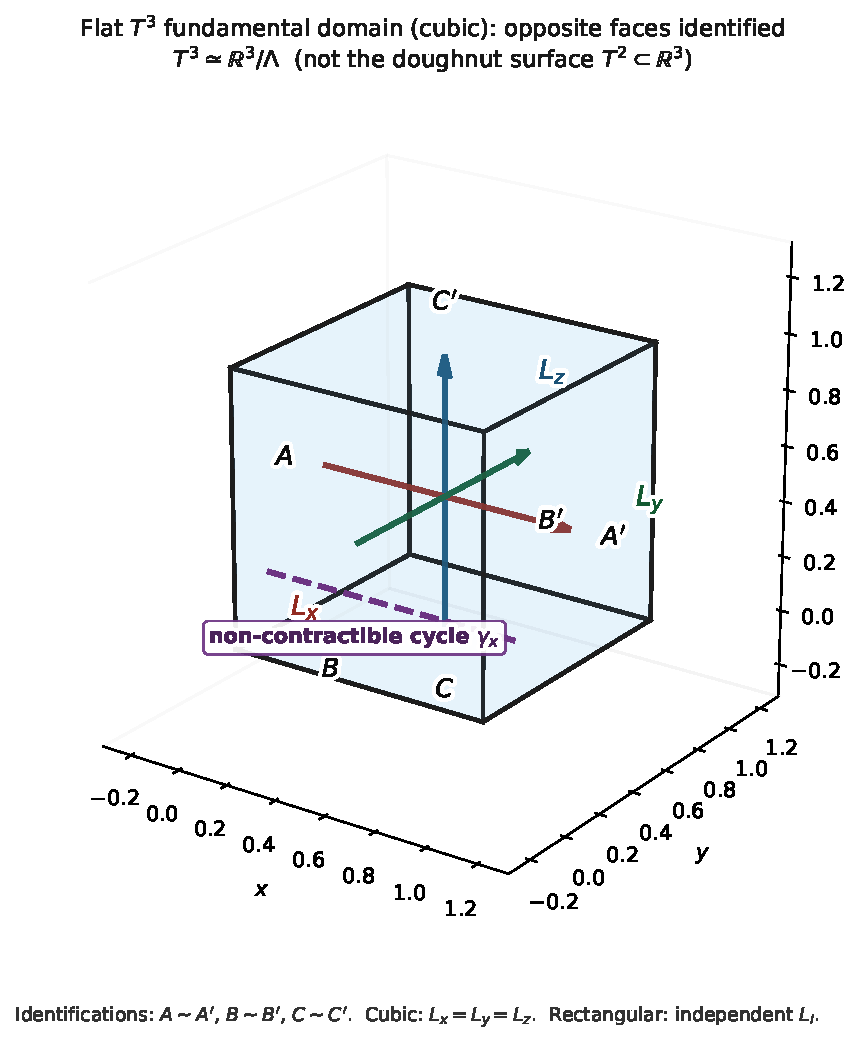
\includegraphics[width=\columnwidth]{itsm_t3_fundamental_domain.pdf}
\caption{Flat cubic \(\Tthree\) fundamental domain: opposite faces identified
(\(A\sim A'\), \(B\sim B'\), \(C\sim C'\)).  Edge lengths \(L_x,L_y,L_z\) are
the three independent periods.  Cubic means \(L_x=L_y=L_z\).  This is not the
embedded doughnut \(\Ttwo\).}
\label{fig:t3}
\end{figure}

``\(\Tthree\)'' alone does not imply equal periods.  Isotropic statements
require a \emph{cubic} (or explicitly isotropised) lattice.  Rectangular and
twisted flat manifolds (\(E_2\), \(E_3\), \ldots) are different geometries with
different CMB constraints \cite{planck_topology,compact_promise}.

Throughout, \(L\) means a \emph{physical} edge length at the epoch under
discussion unless ``comoving'' is written explicitly.  When a numerical Hubble
scale is needed we take
\(\Hzero=70\,\mathrm{km\,s^{-1}\,Mpc^{-1}}\) for illustration; none of the
scoped arguments depends on that choice at the factor-of-two level.

% =============================================================================
\section{\texorpdfstring{\(\azero=c\Hzero/2\pi\)}{a0 = c H0 / 2 pi}
is not circulation quantization}
\label{sec:a0}

\paragraph{Requirements (M1)--(M4).}
A circulation-based derivation must first specify a phase-bearing order
parameter and mass parameter, obtain integer winding, fix the physical
meaning of \(L\), and derive its map to \(\azero\).  The requirements in
Sec.~\ref{sec:path} are the standard for the following test, rather than
assumptions that the kinematic assignment already satisfies.

\subsection{What quantization requires}

For a neutral nonrelativistic superfluid with order parameter
\(\Psi=\sqrt{n_s}\,e^{i\theta}\), the velocity is
\(\mathbf v=(\hbar/m)\nabla\theta\), giving
\begin{equation}
  \Gamma = \oint \mathbf{v}\cdot d\mathbf{l}
  = w\,\frac{h}{m}\,,
  \qquad w\in\mathbb{Z}\,,
  \label{eq:true-quant}
\end{equation}
with single-valuedness of \(\Psi\) on closed cycles
\cite{onsager,feynman,volovik}.  Equation~\eqref{eq:true-quant} quantizes
\emph{phase winding}, not ``length times a speed limit.''
Relativistic circulation concerns the appropriate canonical momentum; this
nonrelativistic velocity formula cannot justify a massive flow at \(v=c\).

\subsection{The author-defined circulation hypothesis}

The hypothesis introduces
\begin{equation}
  \kappa_{\mathrm{cosmo}} \stackrel{?}{=} c\,L
  \label{eq:fake-kappa}
\end{equation}
by multiplying a maximum speed by a length.  For constant speed on a cycle of
length \(L\), one has only \(\Gamma=vL\); setting \(v=c\) yields \(\Gamma=cL\).
No integer winding, no order parameter, and no mass \(m\) enter.  That is a
kinematic assignment, not quantization.

If one formally equated the \(w=1\) nonrelativistic quantum to \(c^{2}/\Hzero\),
\begin{equation}
  m = \frac{h\Hzero}{c^{2}}
  \sim 10^{-32}\,\mathrm{eV}/c^{2}\,,
  \label{eq:mass-pred}
\end{equation}
one would impose a microscopic mass relation, not eliminate microphysics.
This algebraic identification is not a relativistic flow solution or a
derived particle-mass prediction.

\subsection{Internal inconsistency of the \texorpdfstring{\((L,\Gamma,\omega)\)}{(L, Gamma, omega)} package}

Let \(s\) denote physical arclength on a closed cycle of length
\(L=c/\Hzero\). Define a cycle clock by
\(\varphi=2\pi s/L\), so \(\omega=\dot\varphi=2\pi v/L\) for uniform
motion at the epoch in question. Then:
\begin{itemize}
\item \(\Gamma=cL\) implies \(v=c\);
\item \(\omega=\Hzero\) implies
  \(v=\Hzero L/(2\pi)=c/(2\pi)\), contradicting \(v=c\).
\end{itemize}
Thus one cannot simultaneously maintain
\begin{equation}
  L=\frac{c}{\Hzero}\,,
  \qquad
  \Gamma=cL\,,
  \qquad
  \omega=\Hzero
  \label{eq:inconsistent}
\end{equation}
under that cycle-clock definition. A closed geodesic of a flat torus has
zero intrinsic covariant acceleration. Its periodic coordinate does not
create an embedded circular orbit or a centripetal force \(v^2/[L/(2\pi)]\).
No such force is used in this consistency test. ``Distributing \(c\Hzero\) across a
\(2\pi\) angular topology'' is not coordinate-invariant: the range of an
angular chart can be rescaled.  A physical \(2\pi\) arises only from a defined
phase convention coupled to velocity.

\paragraph{Conclusion.}
\begin{equation}
  \azero \equiv \frac{c\Hzero}{2\pi}
  \label{eq:a0-phen}
\end{equation}
may be retained only as a \emph{present-epoch phenomenological scale-matching
postulate} that encodes Eq.~\eqref{eq:coincidence}.  For
\(\Hzero=70\,\mathrm{km\,s^{-1}\,Mpc^{-1}}\) one finds
\(\azero\approx 1.1\times 10^{-10}\,\mathrm{m\,s^{-2}}\), of the observed
order of magnitude \cite{mcgaugh_rar}.  Under the assumptions tested here,
``geometric derivation from circulation quantization'' is unsupported unless
the microphysical requirements (M1)--(M4) are supplied.

% =============================================================================
\section{The projector ratio does not determine
\texorpdfstring{\(\Cobs\)}{C\_obs}}
\label{sec:proj}

\paragraph{Requirements (E1) and (E3).}
A geometric coefficient must be traced through an action and matter coupling
to a physical force.  If the projector is essential, its role and dynamics
must be specified before extracting \(\Cobs\), as required by (E1).
Compact-source integrability and solved periodic fields remain the separate
requirement (E3).  The trace identity and the static action below distinguish
these tasks from a count of tensor components.

\subsection{The identity}

For any \(n^{i}\) with \(\gamma_{ij}n^i n^j=1\), define the metric
trace by \(\operatorname{Tr}_{\gamma}(h)=\gamma^{ij}h_{ij}\). Then
\begin{equation}
  h_{ij}=\gamma_{ij}-n_{i}n_{j}\,,
  \qquad
  \frac{\operatorname{Tr}_{\gamma}(h)}{\operatorname{Tr}_{\gamma}(\gamma)}
  =\frac{2}{3}\,.
  \label{eq:trace}
\end{equation}
This is correct, topology-independent, and independent of superfluidity.  It
discards tensorial orientation information and is not special to \(\Tthree\).

\subsection{Static AQUAL-type action}

A static AQUAL-type force sector \cite{bekenstein_milgrom} may be written
\begin{align}
  S_{\mathrm{WF}}
  &= \int\! dt\,d^{3}x
  \Biggl[
  -\frac{|\nabla\Phi_{N}|^{2}}{8\pi G}
  - \rho_{b}\Phi_{N}
  \nonumber\\
  &\qquad
  - \frac{\CIR}{12\pi G\,\azero}\,|\nabla\psi|^{3}
  - \Cm\,\rho_{b}\,\psi
  \Biggr]\,,
  \label{eq:SWF}
\end{align}
Here \(\azero>0\), \(\Cm>0\), and \(\CIR>0\) define the attractive
positive-coefficient branch used below. The potentials have dimensions
\([\Phi_N]=[\psi]=\mathrm{L}^2\mathrm{T}^{-2}\), so
\([|\nabla\psi|]=[\azero]=\mathrm{L}\mathrm{T}^{-2}\), while \(\Cm\)
and \(\CIR\) are dimensionless. Write
\(q=|\nabla\psi|=\sqrt{\gamma^{ij}\partial_{i}\psi\partial_{j}\psi}\).
Neither \(n^{i}\) nor \(h_{ij}\) appears.  The kinetic operator is fully
three-dimensional and isotropic.  There is therefore no field-theoretic sense
in which Eq.~\eqref{eq:trace} ``matches'' onto the EFT.

Variation yields
\begin{equation}
  \nabla\cdot\!\left(\frac{|\nabla\psi|}{\azero}\,\nabla\psi\right)
  = 4\pi G\,\frac{\Cm}{\CIR}\,\rho_{b}\,.
  \label{eq:p3}
\end{equation}
In spherical symmetry, with \(g_{N}=|\nabla\Phi_{N}|\) and physical
acceleration \(g_{P}=\Cm|\nabla\psi|\),
\begin{equation}
  g_{P} = \Cobs\sqrt{\azero\,g_{N}}\,,
  \qquad
  \boxed{
  \Cobs = \frac{\Cm^{3/2}}{\sqrt{\CIR}}
  }\,.
  \label{eq:Cobs}
\end{equation}

\subsection{Field-rescaling invariance}

Under \(\psi\mapsto s\psi\) with \(s>0\),
\begin{equation}
  \Cm\mapsto\frac{\Cm}{s}\,,
  \qquad
  \CIR\mapsto\frac{\CIR}{s^{3}}\,,
  \label{eq:rescale}
\end{equation}
while \(\Cobs\) is invariant.  More generally, an invariant monomial obeys
\(-a-3b=0\) for \(\Cm^a\CIR^b\); the response in
Eq.~\eqref{eq:Cobs} is the positive square root of the corresponding basic
ratio \(\Cm^3/\CIR\).  Setting \(\Cm=\CIR\) so that \(\Cobs=C\) is a
normalization convention, not a calculation of \(C=2/3\).

Field-rescaling invariance does not make \(\Cobs\) separately identifiable
when the acceleration scale is also free. In the spherical force the
dimensional combination is
\begin{equation}
 a_{0,\mathrm{eff}}=\frac{\Cm^3}{\CIR}\azero=\Cobs^2\azero.
 \label{eq:identifiable-scale}
\end{equation}
Indeed, \(\azero\mapsto\lambda\azero\) and
\(\CIR\mapsto\lambda\CIR\), with dimensionless \(\lambda>0\), leave
Eq.~\eqref{eq:SWF} unchanged while
\(\Cobs\mapsto\Cobs/\sqrt{\lambda}\). A separate numerical \(\Cobs\)
therefore needs an independently fixed \(\azero\) and matching convention;
the spherical response alone cannot measure both.

\paragraph{Scope of the result.}
Equation~\eqref{eq:trace} alone does not support a statement that
\(\Cobs=2/3\) follows from \(\Tthree\) geometry or from ``matching.''  Such a
derivation would require inserting \(h^{ij}\) into the action, specifying its
dynamical origin, and integrating out the relevant fields.

\subsection{Compact sources}

On compact \(\Tthree\), the integral of any pure divergence vanishes, so
localized solutions must use a compensated density contrast (and, if present,
a zero-mean exchange source).  For a flat periodic metric, general morphology,
and the local-static baseline with vanishing exchange source,
\begin{equation}
  \frac{|\nabla\psi|}{\azero}\,\nabla\psi
  = \frac{\Cm}{\CIR}\,\nabla\Phi_{N} + \nabla\times\mathbf{H}
    + \mathbf{h}_0\,,
  \label{eq:curl}
\end{equation}
where \(\mathbf H\) is periodic and \(\mathbf h_0\) is the constant harmonic
flux fixed by the solution.  A periodic curl has zero spatial mean, but the
nonlinear gradient flux need not, so dropping \(\mathbf h_0\) needs an
additional condition.  It is not a freely fitted uniform acceleration.
A nonzero exchange source requires its own source contribution before the
difference is divergence-free; a curved metric requires the corresponding
metric-dependent Hodge decomposition. A pointwise square-root formula is not
a general identity for disks; its accuracy requires a solved field equation.
Neither this decomposition nor compact topology
derives \(\Cobs=2/3\).

% =============================================================================
\section{Present-epoch matching versus fixed-comoving FLRW}
\label{sec:dynamic}

\paragraph{Requirement (S1).}
A viable scale construction must distinguish a present-epoch identification
from a dynamical length history.  If the latter is intended, it must provide
the corresponding modulus dynamics.  The following calculation tests exact
Hubble tracking with fixed comoving moduli.

For fixed comoving moduli \(L^{\mathrm{(com)}}\),
\begin{equation}
  L_{\mathrm{phys}}(t)=a(t)\,L^{\mathrm{(com)}}\,,
  \qquad
  \frac{\dot L_{\mathrm{phys}}}{L_{\mathrm{phys}}}=H\,.
  \label{eq:fixed}
\end{equation}
Requiring instead \(L_{\mathrm{phys}}(t)=c/H(t)\) gives
\begin{equation}
  \frac{\dot L_{\mathrm{phys}}}{L_{\mathrm{phys}}}
  = -\frac{\dot H}{H}\,,
  \label{eq:dsm-rate}
\end{equation}
and equating the two yields \(\dot H=-H^{2}\), i.e.\ deceleration parameter
\(q=0\) (coasting).  Exact tracking is therefore incompatible with ordinary
matter-, radiation-, or \(\Lambda\)-dominated FLRW evolution under fixed
comoving moduli.

The remaining alternatives are: (i)~present-epoch numerical identification
only; or (ii)~an independent modulus sector with its own kinetic term and
stress-energy.  No such sector is constructed here.

The Hubble sphere \(c/H\) is also not generally a particle or event horizon;
calling it a ``global causal domain'' therefore requires an additional causal
definition \cite{davis_lineweaver_horizon}.

% =============================================================================
\section{Cubic topology bounds and \texorpdfstring{\(L=c/\Hzero\)}{L = c/H0}}
\label{sec:bounds}

\paragraph{Requirement (S2).}
The global length must also satisfy topology constraints evaluated for the
same declared background and statistic.  This test is separate from the
modulus-history requirement in Sec.~\ref{sec:dynamic}; the benchmark below
does not turn a background-dependent bound into a universal exclusion.

Planck topology analyses constrain cubic \(E_1\) three-tori within the
background and signal models used in those analyses. In terms of the radius
\(R_i\) of the largest sphere inscribed in the fundamental domain, the
likelihood analysis reports \(R_i>0.97\,\chi_{\mathrm{rec}}\) at a
log-likelihood-ratio threshold \(\Delta\ln\mathcal L>-5\) relative to the
simply connected flat Planck best-fit model \cite{planck_topology}.
The polarization matched-circles search gives the same numerical radius
limit at 99\% confidence; these are distinct statistics, not interchangeable
confidence statements. For a cube of side \(L\),
\(R_i=L/2\), so
\begin{equation}
  L \gtrsim 1.94\,\chi_{\mathrm{rec}}\,.
  \label{eq:L-chi}
\end{equation}
The cited Planck 2018 TT,TE,EE+lowE+lensing central values are
\(r_*=144.43\,\mathrm{Mpc}\), \(100\theta_*=1.04110\), and
\(\Hzero=67.36\,\mathrm{km\,s^{-1}\,Mpc^{-1}}\) \cite{planck}.
On that flat background
\(\chi_{\mathrm{rec}}=r_*/\theta_*\). With
\(c=299792.458\,\mathrm{km\,s^{-1}}\),
\begin{align*}
\theta_* &= 0.0104110,\\
\chi_{\mathrm{rec}}
 &= 144.43/0.0104110 = 13872.8\,\mathrm{Mpc},\\
c/\Hzero
 &= 299792.458/67.36 = 4450.60\,\mathrm{Mpc},\\
\chi_{\mathrm{rec}}/(c/\Hzero) &= 3.117,\\
1.94\times 3.117 &= 6.05.
\end{align*}
The central-value product is therefore
\(L\gtrsim 6.05\,c/\Hzero\). The retained conversion
\begin{equation}
  L \gtrsim 6\,\frac{c}{\Hzero}
  \label{eq:L-H}
\end{equation}
rounds that product to the one-figure \(\mathcal{O}(6)\) bound already
stated in the abstract. It is an approximate conversion in the cited
background, not a topology-only inequality in Hubble units. The coarser
round number \(3.15\) is not the ratio obtained from these central values.
The \(\mathcal{O}(6)\) statement, the factor-of-six comparison below, and
Eq.~\eqref{eq:a0-suppressed} are unchanged. Recent topology surveys likewise place the shortest
\(E_1\) side near the diameter scale of the last-scattering surface, not one
Hubble radius \cite{compact_promise,planck_topology}.

Write \(L=\alpha\,c/\Hzero\).  Empirical scale matching uses \(\alpha=1\);
cubic bounds in the stated benchmark require \(\alpha\gtrsim\mathcal{O}(6)\). If the phenomenological
formula is reinterpreted as \(\azero=c^{2}/(2\pi L)=c\Hzero/(2\pi\alpha)\),
an \(\alpha\) satisfying that benchmark bound yields
\begin{equation}
  \azero \lesssim \frac{1}{6}\times\frac{c\Hzero}{2\pi}
  \sim 1.8\times 10^{-11}\,\mathrm{m\,s^{-2}}\,,
  \label{eq:a0-suppressed}
\end{equation}
which no longer reproduces the intended MOND-scale match.  Therefore the
cubic-\(E_1\), \(\alpha=1\) package fails that simultaneous scale-matching
and topology benchmark.

Vague statements that a ``Hubble-scale domain is compatible with non-detection''
are not supported for cubic \(E_1\) under these bounds.
An altered expansion history, recombination distance, or CMB transfer model
requires recomputing the distance conversion and applicable likelihood;
the factor of approximately six is not an all-cosmology exclusion of \(T^3\).

% =============================================================================
\section{Conditional RAR normalization check in the spherical baseline}
\label{sec:rar}

\paragraph{Requirement (E2).}
The matched response must retain the intended RAR/BTFR normalization.
This final check connects the proposed geometric inputs to their consequence
for the analytic force and velocity normalization.

This section is deliberately conditional.  It uses the static AQUAL-type
action of Eq.~\eqref{eq:SWF}, the positive-mass spherical branch, regular-origin
flux, and no added homogeneous flux.  It then imposes \(\Cobs=2/3\) as a
comparator; Sec.~\ref{sec:proj} does not derive that value.  The result is
therefore neither a global periodic-\(\Tthree\) solution nor a disk-galaxy fit.

In the deep-MOND regime, \(g_{P}=\Cobs\sqrt{\azero g_{N}}\) is equivalent to
\begin{equation}
  g_{P}=\sqrt{a_{0,\mathrm{eff}}\,g_{N}}\,,
  \qquad
  a_{0,\mathrm{eff}} = \Cobs^{2}\,\azero\,.
  \label{eq:a0eff}
\end{equation}
Imposing both \(\azero=c\Hzero/2\pi\approx 1.1\times 10^{-10}\,\mathrm{m\,s^{-2}}\)
and \(\Cobs=2/3\) yields
\begin{equation}
  a_{0,\mathrm{eff}} = \frac{4}{9}\azero
  \approx 4.8\times 10^{-11}\,\mathrm{m\,s^{-2}}\,,
  \label{eq:a0eff-num}
\end{equation}
whereas modern RAR determinations find
\(a_0\simeq 1.2\times 10^{-10}\,\mathrm{m\,s^{-2}}\)
\cite{mcgaugh_rar,lelli_rar}, a factor \(\sim 2.5\) normalization difference
under these assumptions.
In the asymptotic deep-MOND spherical baseline,
\(v^{4}\propto \Cobs^{2}\azero GM_{b}\). At fixed input \(\azero\) and
baryonic mass, the unit-response comparator gives
\begin{equation}
 \frac{v(\Cobs=2/3)}{v(\Cobs=1)}
 =\sqrt{\frac{2}{3}}\simeq0.8165.
 \label{eq:velocity-comparator}
\end{equation}
The approximately 18\% reduction is specifically this same-scale comparator;
it does not use the empirical reference
\(a_{\rm emp}=1.2\times10^{-10}\,\mathrm{m\,s^{-2}}\). For that distinct
reference and the illustrative \(\Hzero=70\) input, the velocity ratio is
\(\bigl[a_{0,\mathrm{eff}}/a_{\rm emp}\bigr]^{1/4}\simeq0.7957\), or a
reduction of about 20.4\%. These are analytic comparators, not observed
discrepancies or completed empirical rejections.

Within this branch, one cannot simultaneously identify
\(\azero=c\Hzero/2\pi\) with the empirical MOND scale and impose a universal
\(\Cobs=2/3\) without changing the effective normalization.  Consistent
options for a future fit are:
\begin{enumerate}
\item set \(\Cobs=1\) (up to the definition of \(\azero\));
\item redefine the input scale so that \(\Cobs^{2}\azero\) matches the RAR;
\item drop universality and derive a morphology-dependent response from a
  solved disk PDE before fitting.
\end{enumerate}

This note stops at analytic normalization. It contains no data likelihood,
nuisance marginalization, intrinsic-scatter test, or model evidence. Such
inferences require a follow-up with a specified geometry-dependent response,
matching inputs, data selection, and nuisance model.

% =============================================================================
\section{Evaluation criteria, retained results, and a reconstruction path}
\label{sec:path}

\subsection{What this note establishes}

\begin{enumerate}
\item The coincidence \eqref{eq:coincidence} is empirical motivation only.
\item \(\azero\equiv c\Hzero/2\pi\) is allowed solely as a
  \emph{present-epoch phenomenological postulate}.
\item The weak-field combination
  \(\Cobs=\Cm^{3/2}/\sqrt{\CIR}\) is a derived, normalization-invariant
  response coefficient at fixed \(\azero\) [Eq.~\eqref{eq:Cobs}]; without that
  choice the spherical force identifies only \(\Cobs^2\azero\).
\item On compact \(\Tthree\), sources must be compensated and disk solutions
  generally admit a curl term [Eq.~\eqref{eq:curl}].
\item The scoped incompatibilities in Secs.~\ref{sec:a0}--\ref{sec:rar}
  constrain the tested cubic geometric packaging of those two numbers without
  deciding MOND or alternative microscopic constructions as a class.
\end{enumerate}

\subsection{Path required before any geometric-derivation claim}

A subsequent work that claims to \emph{derive} \(\azero\) or \(\Cobs\) from
topology or microphysics must close the following chain.  Items are grouped
by sector, and each is a separately testable technical requirement.

\paragraph{Microphysics and circulation.}
\begin{enumerate}
\item[(M1)] Define a condensate order parameter
  \(\Psi=\sqrt{\rho}\,e^{i\theta}\)
  (or a relativistic analogue) with a definite mass parameter \(m\).
\item[(M2)] Obtain the circulation from \(\nabla\theta\) and impose integer
  winding on non-contractible cycles of \(\Tthree\), yielding
  \(\Gamma=w\,h/m\) in the nonrelativistic limit rather than \(\Gamma=cL\).
\item[(M3)] Fix a single geometric meaning of \(L\)
  (cube edge, closed geodesic length, or circumference) and use it
  consistently in every formula.
\item[(M4)] Derive a map
  \((\Gamma,m,w,L)\mapsto\azero\)
  that does not rely on a chart-dependent ``distribution'' of \(c\Hzero\) over
  an angular range of \(2\pi\).
\end{enumerate}

\paragraph{Cosmic scale and moduli.}
\begin{enumerate}
\item[(S1)] Either restrict scale matching to the present epoch, or supply a
  modulus action for \(L_{\mathrm{phys}}(t)\) that does not force the
  coasting condition \(q=0\).
\item[(S2)] Confront the resulting \(L\) with Planck/COMPACT bounds for cubic
  \(E_1\) and for twisted flat alternatives \cite{planck_topology,compact_promise}.
\end{enumerate}

\paragraph{Weak-field coefficient and data.}
\begin{enumerate}
\item[(E1)] If a projector \(h_{ij}\) is essential, insert it into the action,
  specify the dynamics of \(n^{i}\), and compute
  \(\Cobs=\Cm^{3/2}/\sqrt{\CIR}\)
  as a definite number independent of field normalization.
\item[(E2)] Reconcile \(\Cobs^{2}\azero\) with the empirical RAR/BTFR
  normalization, accounting for the conditional factor \(4/9\) in
  Sec.~\ref{sec:rar} rather than treating it as an independent data rejection.
\item[(E3)] Solve the compensated periodic nonlinear equation for at least one
  locally spherical and one disk baryonic source, including curl and harmonic
  contributions; periodicity does not supply global spherical symmetry.
\end{enumerate}

\paragraph{Representation (already satisfied here).}
\begin{enumerate}
\item[(R1)] Use a face-identified parallelepiped for \(\Tthree\)
  (Fig.~\ref{fig:t3}), never an embedded doughnut \(\Ttwo\).
\end{enumerate}

Absent evidence closing (M1)--(M4), (S1)--(S2), and (E1)--(E3), this note
supports present-epoch phenomenological matching of
Eq.~\eqref{eq:coincidence}, the derived invariant \(\Cobs\), and the scoped
constraints on the tested cubic construction---not a geometric derivation of
the MOND scale.

% =============================================================================
\section*{Code and data availability}

\begingroup
\raggedright
Figure~\ref{fig:t3} is produced by
\texttt{Scripts/itsm\_t3\_fundamental\_domain.py}.
Source code is available in the
\href{https://github.com/brendohxd/ITSM-Integrated-Toroidal-Syntropic-Model}{public GitHub repository}
and the \href{https://doi.org/10.5281/zenodo.18808348}{Zenodo record 10.5281/zenodo.18808348}.
That record is the historical public archive of the v11 package
constrained in this note. It is not a derivation authority.
Scripts that render an embedded doughnut surface depict \(\Ttwo\) and should
not be used as \(\Tthree\) schematics.  No new observational catalogue is
analysed.
\par
\endgroup

\section*{Declaration on the use of artificial-intelligence tools}

Artificial-intelligence-assisted tools were used for editorial drafting,
source-code assistance, and checks of symbolic and numerical consistency.
This local review draft still requires the author's final verification of
the manuscript, equations, cited sources, and generated artifacts. Submission
requires the author's confirmation of that review and acceptance of full
responsibility; neither is certified by these automated checks.

\bibliography{references}

\end{document}
